\documentclass[a4paper,10pt,english]{scrartcl}
\usepackage{mystyle}
% Title Page
\title{Machine Learning Project 2010--2011}
\subtitle{Meta-learning from an experiment database}
\author{Jonas De Greef\and Li Quan}
\date{}

\newcommand{\dataset}[1]{\emph{#1}}

\begin{document}
\maketitle
\begin{abstract}
For the machine learning project, we will study meta-learning from an experiment database\cite{Blockeel06-KDID:proc,42686}.% in order to understand and use machine learning algorithms better.
\end{abstract}


\section{Introduction}
In our introductory paper we put our main focus on large datasets and we wanted to study the effects of noise, parameters and other effects of working with larger datasets.
Due to the relatively low amount of datasets of large size and also the rather few experiments performed on these datasets, we've had to make some explicit choices of which data to process and what points of interest to explore further.

A first limitation is that we will only study datasets larger than 5000: the datasets in the database are given in \autoref{tab:datasets}. Unfortunately, these datasets cannot truly be said to be 'large', but rather mediocre in size. Still, we hope when focussing on at least these 11 largest of the given datasets that we will be able to make reasonable assumptions concerning the algorithms used and the effects of noise and parameters.

\begin{table}[hbpt]
\centering\footnotesize
\begin{tabular}{l r }
\toprule
Dataset name    & Size          \\\midrule
waveform-5000	& 5000            \\
page-blocks     & 5473          \\
optdigits	    & 5620            \\
satimage	    & 6430         \\
mushroom	    & 8124         \\
pendigits       & 10992         \\
nursery	        & 12960         \\
letter	        & 20000          \\
kropt	        & 28056        \\
adult	        & 48842           \\
covertype	    & 110393          \\

\bottomrule
\end{tabular}
\caption{Datasets with size greater than 5000.}
\label{tab:datasets}
\end{table}

\section{Initial impressions}
We will start off with some initial impressions concerning the datasets we will be handling and the algorithms we will be evaluating on them.
First of all, the average accuracy of all algorithms applied to these datasets is given in \autoref{fig:pred_acc}: this graph does not take in account the number of datasets, e.g., weka.Winnow has an (average) predictive accuracy of $0.99$---but this is the result of only 1~dataset where 22~experiments were performed, so this algorithm is not as interesting as it might seem. Still, it seems that quite a few algorithms perform quite well on these 'larger' datasets, some of which we will discuss more in-depth later. Similarly, the inverse graph \autoref{fig:pred_acc_data}: where we plot the average predictive accuracy over all algorithms for each dataset shows us that \dataset{kropt} is not an easy dataset to model. Also, a clear trend is visible in such that the larger the dataset the less accurate the algorithms generally perform.
\begin{figure}[hbpt]
\centering
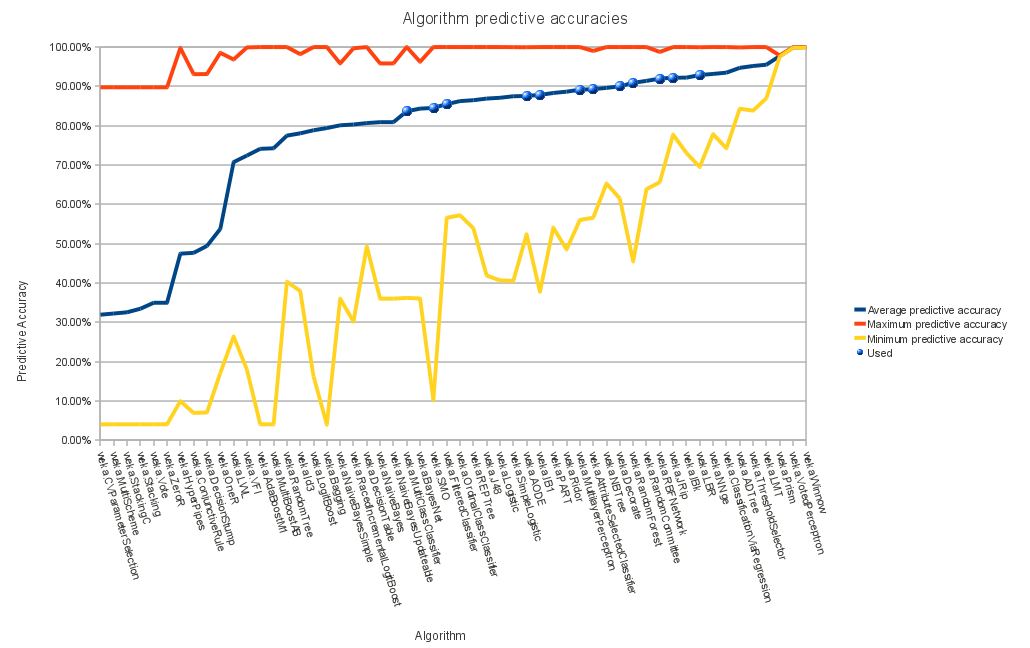
\includegraphics[width=\textwidth]{pred_acc}
\caption{Predictive accuracy of all algorithms on datasets with size greater than 5000.}
\label{fig:pred_acc}
\end{figure}
\begin{figure}[hbpt]
\centering
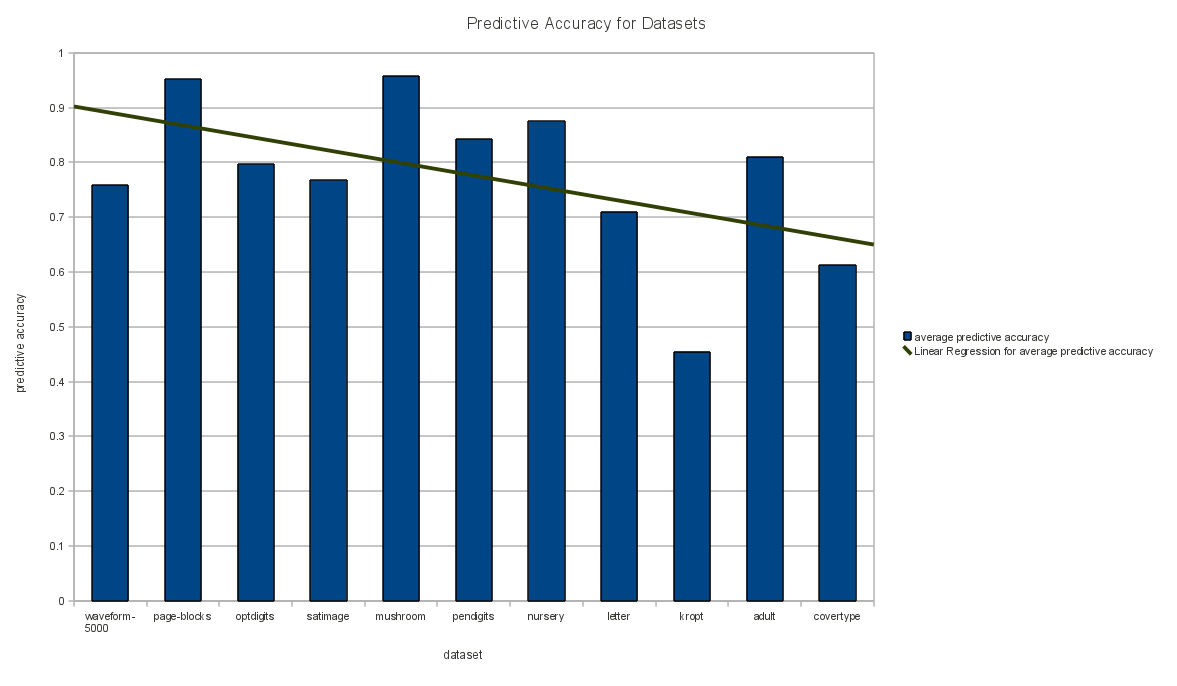
\includegraphics[width=\textwidth]{pred_acc_data}
\caption{Predictive accuracy of all datasets with size greater than 5000 on all algorithms.}
\label{fig:pred_acc_data}
\end{figure}

Second, we decided to filter out some algorithms with a high average accuracy (namely greater than 80 percent), applied on at least half of all eligible datasets and at least an average of 10 experiments per dataset. This way we try to assemble a small amount of algorithms which we (hopefully) can study much closer for the effects of their parameters and their performances on the chosen datasets. The chosen algorithms are both shown in \autoref{fig:pred_acc} (the blue dots) and in \autoref{tab:algorithms}.

\begin{table}[hbpt]
\centering\footnotesize
\begin{tabular}{l r r r l}
\toprule
Algorithm  & \# Datasets & \# Experiments & Pred.\ Accuracy & Type \\\midrule
weka.JRip&	9	&157&	0.90 & Rule Learner\\
weka.RandomCommittee&	9&	168&	0.90 &Ensemble\\
weka.Decorate	&	8	&175&0.90&Ensemble\\
weka.MultilayerPerceptron	&11	&3037 &	0.88&Neural Network\\
weka.RBFNetwork		&9	&141&0.88&Neural Network\\
weka.RandomForest		&11&	980&0.88&Decision Tree\\
weka.PART	&	10&	183 &0.88&Decision List\\
weka.J48		&11&	7615 &0.86&Decision Tree\\
weka.REPTree		&11	&187 &0.86&Decision Tree\\
weka.MultiClassClassifier&	11	&184 &	0.83&Meta\\
weka.LogitBoost		&11&	1615&0.83&Regression Learner\\
weka.SMO		&11&	6656 & 0.82&Support Vector Machine\\
\bottomrule
\end{tabular}
\caption{Algorithms with high predictive accuracy, tested on more than 5 datasets and for each dataset a minimum of 10 experiments.}
\label{tab:algorithms}
\end{table}

Third, \autoref{fig:time_memory} shows the time and memory usage for the algorithms. As expected, in general the build stage is less time and memory consuming than the run stage. A distinct impression is that the Decision Tree-algorithms seem to use much less CPU and relatively fewer memory than the other algorithms. This was a predictable result but it highlights that these algorithms will probably be some of the most prominent challengers when it comes down to handling large datasets when it comes down to efficiency.

Fourth, we cannot offer an initial impression concerning the influence of noise since the datasets do not share how much noise they include. We will however add noise of ourselves and study the effects on a few of the more interesting algorithms.
\begin{figure}[hbpt]
\centering
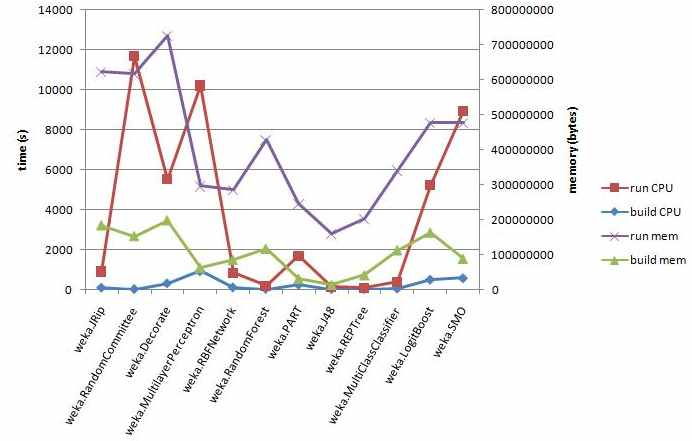
\includegraphics[width=\textwidth]{build_run}
\caption{Time and memory usage (build and run).}
\label{fig:time_memory}
\end{figure}

\section{Experiments}


\begin{lstlisting}

\end{lstlisting}


\section{Conclusion}


\appendix


%% Define a new 'leo' style for the package that will use a smaller font.
\makeatletter
\def\url@leostyle{%
  \@ifundefined{selectfont}{\def\UrlFont{\sf}}{\def\UrlFont{\small\ttfamily}}}
\makeatother
%% Now actually use the newly defined style.
\urlstyle{leo}

\bibliographystyle{acm}
\bibliography{biblio}
\end{document}
